\documentclass[aspectratio=169]{beamer}
\usepackage{appendixnumberbeamer}
\setbeamercovered{transparent=0}
\usetheme[block=fill]{metropolis}

\setsansfont[
    Extension      = .otf,
    UprightFont    = *-Light,
    ItalicFont     = *-LightItalic,
    BoldFont       = *-Regular,
    %BoldItalicFont = *-RegularItalic
]{FiraSans}
\setmonofont[
    Extension   = .otf,
    UprightFont = *-Regular,
    BoldFont    = *-Medium
]{FiraMono}

\title{Eliminating Ghost code}
\subtitle{One step forward, two steps backward}
\author{Noé De Santo}
\date{February 7, 2023}

\usepackage{soul}

\usepackage{dsfont} % \mathds

\newcommand{\true}[0]{\ensuremath{\mathds{1}}}
\newcommand{\false}[0]{\ensuremath{\mathds{O}}}
\usepackage{prftree} % \prftree
\usepackage{extarrows} % \xlongritharrow
\usepackage{tensor} % \tensor
\usepackage{graphicx} % \blacktriangleright
\usepackage{xifthen} % \ifthenelse, \isempty

% Misc
\newcommand{\autopar}[1]{\ifthenelse{\isempty{#1}}{}{\left(#1\right)}}
\newcommand{\pair}[2]{{#1 \circ #2}}
\newcommand{\separator}[0]{\mathrel{\ |\ }}
\newcommand{\defeq}[0]{\mathrel{::=}}
\newcommand{\hole}[0]{[]}
\newcommand{\substitute}[3]{\left[#1 \mapsto #2 \right]#3}
\newcommand{\domain}[1]{\text{dom}\autopar{#1}}
\newcommand{\wildcard}[0]{\raisebox{2pt}{\,\_\,}}
\newcommand{\freevars}[1]{\text{FV}\autopar{#1}}



% Labels/lattice
\newcommand{\labels}[0]{\mathcal{L}}
\newcommand{\glb}[0]{\sqcap}
\newcommand{\lub}[0]{\sqcup}
\newcommand{\lsub}[0]{\sqsubseteq}
\newcommand{\downset}[1]{{#1\!\downarrow}}
\newcommand{\labelof}[1]{\labels{}_\text{of}\!\autopar{#1}}
\newcommand{\labelsin}[1]{\labels{}_\text{in}\!\autopar{#1}}



%\newcommand{\ell}
\newcommand{\emm}[0]{m}
\newcommand{\enn}[0]{n}
\newcommand{\ahh}[0]{h}
\newcommand{\epp}[0]{\rho}



% Types
\newcommand{\constpretype}[0]{\mathcal{C}}
\newcommand{\arrowpretype}[3]{{#1 \xrightarrow{#2} #3}}
\newcommand{\refpretype}[1]{{\textsc{Ref}\ #1}}
\newcommand{\toppretype}[0]{\textsc{Top}}
\newcommand{\type}[2]{\ensuremath{\tensor[_{{#1}}]{{#2}}{}}}
\newcommand{\constype}[1]{\type{#1}{\constpretype}}
\newcommand{\arrowtype}[4]{\type{#1}{\left(\arrowpretype{#2}{#3}{#4}\right)}}
\newcommand{\reftype}[2]{{\type{#1\,}{\refpretype{#2}}}}
\newcommand{\toptype}[1]{\type{#1}{\toppretype}}



% Subtyping
% \newcommand{\tsub}[0]{\ensuremath{\mathrel{\prec:}}}
\newcommand{\atsub}[0]{\ensuremath{\mathrel{<:}}}
\newcommand{\notatsub}[0]{\ensuremath{\mathrel{\mathrlap{<:}{\,\,/}}}}



% Lambda-terms
\newcommand{\typeseparator}[0]{{:}\,}
\newcommand{\typed}[2]{#1\typeseparator{}#2}
\newcommand{\slet}[2]{\texttt{let}\, {#1} = {#2}}
\newcommand{\seq}[2]{{#1;\, #2}}

\newcommand{\abs}[3]{\lambda\typed{#1}{#2}.\ #3}
\newcommand{\app}[2]{#1\,#2}
\newcommand{\deref}[1]{{!#1}}
\newcommand{\enew}[2]{\texttt{new}\left[#1\right]\, #2}
\newcommand{\letseq}[4]{\seq{\slet{\typed{#1}{#2}}{#3}}{#4}}
\newcommand{\asseq}[3]{\seq{{#1} := {#2}}{#3}}

\newcommand{\unit}[0]{()}



% Lambda-reduction
\newcommand{\reduces}[5][]{\pair{#2}{#3} \ \xlongrightarrow{#1} \  \pair{#4}{#5}}
\newcommand{\creduces}[4]{\reduces[*]{#1}{#2}{#3}{#4}} % Closure reduction
\newcommand{\mreduces}[4]{\reduces[=]{#1}{#2}{#3}{#4}} % Maybe reduction
% \newcommand{\sreduces}[4]{\reduces[+]{#1}{#2}{#3}{#4}} % Sequence reduction



% Lambda-equivalence, normal form...
\newcommand{\normalform}[2][]{{{#2}\downarrow^{#1}}}
\newcommand{\obsequiv}[0]{\equiv}



% Context ops
\newcommand{\supervc}[0]{\supseteq^{\gamma}}
\newcommand{\contextextend}[3]{#1+\enumset{\typed{#2}{#3}}}


% Store ops
\newcommand{\superstore}[0]{\supseteq^{\sigma}}
\newcommand{\storeupdate}[3]{\substitute{#2}{#3}{#1}}
\newcommand{\storeextend}[3]{#1+\left\{#2\mapsto{}#3\right\}}



% Judgments
\newcommand{\arrowvdash}{%
    \mathrel{%
        \vdash\hspace*{-5pt}%
        \raisebox{2.65pt}{\scalebox{.33}{\(\blacktriangleright\)}}%
    }%
}
\newcommand{\storejudgmentscheme}[4]{{\pair{#1}{#2} #4 #3}}
\newcommand{\judgmentscheme}[6]{{\pair{#1}{#2} #6 #3 \ : \pair{#4}{#5}}}
\newcommand{\judgment}[5]{\judgmentscheme{#1}{#2}{#3}{#4}{#5}{\vdash{}}}
\newcommand{\ajudgment}[5]{\judgmentscheme{#1}{#2}{#3}{#4}{#5}{\arrowvdash{}}}
\newcommand{\asjudgment}[3]{\storejudgmentscheme{#1}{#2}{#3}{\arrowvdash{}}}


% Relevance & erasure
\newcommand{\threshold}[0]{\ensuremath{\tau}}
\newcommand{\relevance}[2][\threshold]{\ensuremath{\mathcal{R}^{#1}\!\autopar{#2}}}
\newcommand{\erasure}[2][\threshold]{\ensuremath{\mathcal{E}^{#1}\!\autopar{#2}}}
\newcommand{\eGamma}[0]{\erasure{\Gamma}}
\newcommand{\eSigma}[0]{\erasure{\Sigma}}



% Store extension
%\newcommand{\stextends}[4]{\pair{\pair{#1}{#2}}{#3} \ \rightsquigarrow \ #4}
\newcommand{\extender}{\text{ext}}
\newcommand{\stextends}[2]{\extender^{\sigma}\!\autopar{#1,#2}}
\newcommand{\vtextends}[1]{\extender^{\gamma}\!\autopar{#1}}
\RequirePackage{amsmath}
\RequirePackage{amsmath}
\RequirePackage{cleveref}

\RequirePackage[scale=0.9]{FiraMono}
\RequirePackage{listings}

\renewcommand{\lstlistingname}{Algorithm}
\lstset{
    extendedchars=\true,
    inputencoding=utf8,
    texcl=true,
    escapeinside=``,
    frame=tb,
    basicstyle=\ttfamily,
    keywordstyle=\bfseries,,
    morekeywords={Assuming, Input, Output, Runtime, Space, Success, fun, let, if, then, else, for, in, while, loop, do, return, Initialize, Process, assert, match, case, require, class, object, ensuring, Ghost},
    morecomment=[l]{//},
    numbers=left,
    numberstyle=\ttfamily,
    stepnumber=1,
    xleftmargin=2em,
    framexleftmargin=2em,
    breaklines=true,
    breakatwhitespace,
    % For this project only
    moredelim=**[is][\color{gray}]{\#}{\#},
}
\crefname{lstlisting}{algorithm}{algorithms}

\newcommand{\bigo}[1]{\ensuremath{\mathcal{O}\left(#1\right)}}
\newcommand{\bigomega}[1]{\ensuremath{\Omega\left(#1\right)}}

%% Set definitions
\newcommand{\setbuilder}[2]{\left\{ #1 \mid #2 \right\}}
\newcommand{\enumset}[1]{\left\{ #1 \right\}}
\usepackage{etoolbox}
\usepackage{xifthen}

\newcommand{\powerset}[1]{\mathcal{P}\left( #1 \right)}
\newcommand{\rangeset}[2]{\left[#1, #2\right]}

%% Set operations
\newcommand{\scardinality}[1]{\left|#1\right|}
\newcommand{\sdiff}[0]{\backslash}
\newcommand{\sunion}[0]{\cup}
\newcommand{\sinter}[0]{\cap}
\newcommand{\skleene}[1]{{#1}^{*}}
\newcommand{\scompl}[1]{\overline{#1}}
\newcommand{\sUnion}[0]{\bigcup\limits}
\newcommand{\sInter}[0]{\bigcap\limits}

%% Common sets
\newcommand{\N}[0]{\mathbb{N}}
\newcommand{\Z}[0]{\mathbb{Z}}
\newcommand{\R}[0]{\mathbb{R}}

\newcommand{\srangelo}[2]{{\left[#1,\:#2\right[}}

%% List
\def\@cms<#1,#2><#3>{#1\ifthenelse{\isempty{#2}}{}{#3\@cms<#2><#3>}}
\newcommand{\commasep}[2][,\,]{\@cms<#2,><#1>}

\newcommand{\sarray}[1]{\left[ \commasep{#1} \right]}
\newcommand{\slist}[1]{\commasep[\,::\,]{#1}}

\newcommand{\slistindexing}[2]{\left(#1\right)\left[#2\right]}
\lstset{
    frame=,
    commentstyle=\color{mLightGreen},
    moredelim=**[is][\color{mLightBrown}]{\#}{\#},
    moredelim=**[is][\color{red}]{\#-}{\#-},
    moredelim=**[is][\color{gray}\itshape]{\#!}{\#!},
    literate={:N}{$\nats$}{1} {\\}{$\lambda$}{1} {->}{$\rightarrow$}{2}
}

\usepackage{etoolbox}
\usepackage{array}
\usepackage{tikz}
\usetikzlibrary{calc,fit,decorations.pathreplacing,calligraphy}

\newcommand{\sectionimg}[0]{}
\defbeamertemplate{section page}{custom}{
    \centering
    \begin{minipage}{22em}
        \raggedright
        \usebeamercolor[fg]{section title}
        \usebeamerfont{section title}
        \insertsectionhead\\[-1ex]
        \usebeamertemplate*{progress bar in section page}
        \par
        \ifx\insertsubsectionhead\@empty\else%
            \usebeamercolor[fg]{subsection title}%
            \usebeamerfont{subsection title}%
            \insertsubsectionhead
        \fi
    \end{minipage}
    \par
    \ifdefempty{\sectionimg}{ 
        \vspace{\baselineskip}
    }{
        \begin{center}
            \includegraphics[width=22em]{\sectionimg} 
        \end{center}
        \renewcommand{\sectionimg}[0]{}
    }
}
\setbeamertemplate{section page}[custom]
\let\sectionbase\section
\renewcommand{\section}[2][]{\renewcommand{\sectionimg}{#1}\sectionbase{#2}}

\begin{document}

\maketitle

\section[imgs/why.png]{Ghost code?}

\begin{frame}[fragile]{A sparse matrix}
\begin{lstlisting}
class SparseMatrix {
    let data: Repr

    fun * (that: SparseMatrix): SparseMatrix {
        let resData = ... // Do the sparse multiplication
        return SparseMatrix {
            data = resData,
        }
    }
}
\end{lstlisting}
\end{frame}

\begin{frame}[fragile]{\alert{Testing} a sparse matrix}
\begin{lstlisting}
class SparseMatrix {
    let data: Repr
    #let full: Matrix#

    fun * (that: SparseMatrix): SparseMatrix {
        let resData = ... // Do the sparse multiplication
        return SparseMatrix {
            data = resData,
            #full = this.full * that.full#
        }
    }#.ensuring( res => res == SparseMatrix.from(res.full) )#
}
\end{lstlisting}
\end{frame}

\begin{frame}[fragile]{Testing a sparse matrix \alert{for free}}
\begin{lstlisting}
class SparseMatrix {
    let data: Repr
    let full: #Ghost# Matrix

    fun * (that: SparseMatrix): SparseMatrix {
        let resData = ... // Do the sparse multiplication
        return SparseMatrix {
            data = resData,
            full = this.full * that.full
        }
    }.ensuring( res => res == SparseMatrix.from(res.full) )
}
\end{lstlisting}
\end{frame}

\begin{frame}[fragile]{Testing a sparse matrix for free}
\begin{lstlisting}
class SparseMatrix {
    let data: Repr
    #!let full: Ghost Matrix#!

    fun * (that: SparseMatrix): SparseMatrix {
        let resData = ... // Do the sparse multiplication
        return SparseMatrix {
            data = resData,
            #!full = this.full * that.full#!
        }
    }#!.ensuring( res => res == SparseMatrix.from(res.full) )#!
}
\end{lstlisting}
\end{frame}

\begin{frame}[fragile]{\alert{Verifying} a sparse matrix for free}
\begin{lstlisting}
class SparseMatrix {
    let data: Repr
    #!let full: Ghost Matrix#!

    #!@invariant#!
    #!Ghost fun fullMatch(): Ghost Boolean {#!
        #!this == SparseMatrix.from(res.full)#!
    #!}#!

    fun * (that: SparseMatrix): SparseMatrix { ...
    }#!.ensuring( res => res.full == this.full * that.full )#!
}
\end{lstlisting}
\end{frame}

\section{The calculus}

\begin{frame}{Terms}
    \vspace{-0.5em}
    \[
    \begin{array}{rwl{5em}lwc{3em}rwl{7em}l}
        \multicolumn{3}{l}{\textbf{Values}} && \multicolumn{3}{l}{\textbf{Expressions}} \\
        v \defeq & k  & \text{Constant} && \alert<2>{e}\defeq & \app{a}{a} & \text{Application} \\
            \separator \!\!\! & l  & \text{Location} && \separator \!\!\! & \deref{a} & \text{Dereference} \\
            \separator \!\!\! & \abs{x}{T}{p} & \text{Abstraction} && \separator \!\!\! & \enew{T}{a} & \text{Allocation} \\[1em]
        \multicolumn{3}{l}{\textbf{Atoms}} && \multicolumn{3}{l}{\textbf{Let contexts}} \\
        a \defeq & v & \text{Value} && L \defeq & \asseq{a}{a}{L} & \text{Assignment} \\
            \separator \!\!\! & x & \text{Variable} && \separator \!\!\! & \letseq{x}{T}{\alert<2>{e}}{L} & \text{Let-binding} \\
            && && \separator \!\!\! & \hole & \text{Hole} \\[1em]
        \multicolumn{3}{l}{\textbf{Programs}} \only<3->{&& \multicolumn{3}{l}{\textbf{\alert<3>{Terms}\footnotemark}}} \\
        p \defeq & L(a) & \text{Filled context} \only<3->{&& t \defeq & p \separator e}
    \end{array}
    \]
    \only<3->{
        \footnotetext{Note that $v \subset a \subset p$.}
    }
\end{frame}

\begin{frame}{A program}
    \centering
    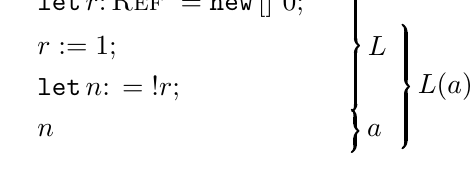
\begin{tikzpicture}
        \useasboundingbox (0,0) rectangle (15em,-5em);

        \tikzstyle{codeline}=[minimum height = 1.5em, text width = 11em, anchor = south west, align = left]

        \node (L1) [codeline] at (0,0) {$\letseq{r}{\refpretype{\nats}}{\enew{\nats}{0}}{}$};
        \node (L2) [codeline] at (0,-1.5em) {$\asseq{r}{1}{}$};
        \node (L3) [codeline] at (0,-3em) {$\letseq{n}{\nats}{\deref{r}}{}$};
        \node (a) [codeline] at (0,-4.5em) {$n$};

        \node (L) [fit = (L1) (L2) (L3), inner sep=0] {};
        \draw<2-> [decoration={calligraphic brace,mirror}, decorate, line width=1.25pt] (L.south east) -- node[right, text width = 1em] (L_label) {$\,L$} (L.north east);
        \draw<2-> [decoration={calligraphic brace,mirror}, decorate, line width=1.25pt] (a.south east) -- node[right] (a_label) {$\,a$} (a.north east);

        \node<2-> (labels) [fit = (L_label) (a_label), inner sep=0] {};
        \draw<2-> [decoration={calligraphic brace,mirror}, decorate, line width=1.25pt] (labels.south east) -- node[right] {$\,L(a) = p$} (labels.north east);
    \end{tikzpicture}
\end{frame}

\begin{frame}{Reduction rules}
\begin{definition}[Reduction derivations]
\begin{gather*}
    \prftree[r]{R-AppAbs}
        {}
        {\reduces{\app{\left(\abs{x}{T}{p}\right)}{v}}{\mu}{\substitute{x}{v}{p}}{\mu}}
    \\[1em]
    \prftree[r]{R-Deref}
        {l \in \domain{\mu}}
        {\reduces{\deref{l}}{\mu}{\mu(l)}{\mu}}
    \qquad
    \prftree[r]{R-Assign}
        {l \in \domain{\mu}}
        {\reduces{\alert<2->{\asseq{l}{v}{p}}}{\mu}{\alert<2->{p}}{\storeupdate{\mu}{l}{v}}}
    \\[1em]
    \prftree[r]{R-New}
        {l \not\in \domain{\mu}}
        {\reduces{\enew{\wildcard}{v}}{\mu}{l}{\storeextend{\mu}{l}{v}}}
    \\[1em]
    \prftree[r]{R-Let}
        {\reduces{e}{\mu}{L(a)}{\mu'}}
        {\reduces{\letseq{x}{T}{e}{p}}{\mu}{L(\substitute{x}{a}{p})}{\mu'}}
\end{gather*}
\end{definition}
\end{frame}

\begin{frame}[fragile]{Calling a function}
\begin{tabular}{wl{12em}>{\onslide<2->}wc{8em}<{\onslide}>{\onslide<2->}l<{\onslide}}
\begin{lstlisting}[boxpos=t]
(\x: :N. 
    let a: :N = 2*x;
    let b: :N = a+3;
    b
)(0)
\end{lstlisting}
&$\xrightarrow{\makebox[4em]{\scriptsize{R-AppAbs}}}$&
\begin{lstlisting}[boxpos=t]
#let a: :N = 2*0;#
#let b: :N = a+3;#
#-b#-
\end{lstlisting}
\end{tabular}

\vspace{1em}
\onslide<3->

\begin{tabular}{wl{12em}>{\onslide<4->}wc{8em}<{\onslide}>{\onslide<4->}l<{\onslide}}
\begin{lstlisting}[boxpos=t]
let n: :N = (\x: :N. 
        let a: :N = 2*x;
        let b: :N = a+3;
        b
    )(0);
r := n;
n
\end{lstlisting}
&$\xrightarrow{\makebox[4em]{\scriptsize{R-Let}}}$&
\begin{lstlisting}[boxpos=t]
#let a: :N = 2*0;#
#let b: :N = a+3;#
r := #-b#-;
#-b#-
\end{lstlisting}
\end{tabular}
\onslide
\end{frame}

\section{Ghost in the calculus}

\begin{frame}{Generalized ghost annotations}
    Every type is annotated with a \alert<1>{(ghost) label}, e.g. $\type{\ell}{\nats}$.
    \vspace{1em}

    \only<2>{
    \begin{definition}[Labels]
        Labels are taken from a bounded lattice $(\labels,\glb,\lub)$. The induced partial order is noted $\lsub$.
    \end{definition}
    }

    \only<3>{
    \begin{block}{Semantic (intuitively)}
    If $\ell \lsub \ahh$:
    \begin{enumerate}
        \item $\ell$ is ``more important'' for run-time than $\ahh$;
        \item ``$\ahh$-annotated data'' cannot flow into ``$\ell$-annotated data''.
    \end{enumerate}
    E.g. $R_{\textsc{egular}} \lsub G_{\textsc{host}}$.
    \end{block}
    }
\end{frame}

\begin{frame}{Typing judgments}
    \begin{definition}[Typing judgment]
        A typing judgment is of the form 
        \[ \ajudgment{\Gamma}{\Sigma}{t}{T}{\ell} \]
    \end{definition}

    \only<1>{
    \begin{itemize}
        \item $\Gamma$: Variable context;
        \item $\Sigma$: Store context;
        \item $t$: Term being typed;
        \item $T$: Determined type;
        \item $\ell$: Determined effect bound.
    \end{itemize}
    }

    \only<2>{
    $\ell$ --- determined effect bound, e.g.:
    \begin{itemize}
        \item $\ell = \top$: No effect;
        \item $\ell = G_{\textsc{host}}$: Only ghost locations are allocated or written to;
        \item $\ell = R_{\textsc{egular}}$: Anything can happen.
    \end{itemize}
    }
\end{frame}

\begin{frame}{Types}
\begin{definition}[Types]
\begin{align*}
    \ell &\in \labels{}
    && \textup{Labels} \\
    P &\defeq \constpretype \separator{} \toppretype \separator{} \refpretype{T} \separator{} \arrowpretype{T}{\alert<2>{\ell}}{T} && \textup{Pre-types} \\
    T &\defeq \type{\ell}{P}
    && \textup{Types}
\end{align*}
\end{definition}
\only<2>{
Bound of the effect of the function \emph{when called}.
}
\end{frame}

% TODO: enable back
\begin{frame}{Typing rules (part 1/$\infty$)}
\begin{definition}[Typing derivations --- atoms]
\begin{gather*}
    \prftree[r]{AT-Var}
        {x \in \domain{\Gamma}}
        {\ajudgment{\Gamma}{\Sigma}{x}{\Gamma(x)}{\top}}
    \qquad
    \prftree[r]{AT-Const}
        {}
        {\ajudgment{\Gamma}{\Sigma}{k}{\constype{\bot}}{\top}}
    \\[0.5em]
    \prftree[r]{AT-Loc}
        {\Sigma(l) = T}
        {\ajudgment{\Gamma}{\Sigma}{l}{\reftype{\labelof{T}}{T}}{\top}}
    \qquad
    \prftree[r]{AT-Abs}
        {\ajudgment{\contextextend{\Gamma}{x}{S}}{\Sigma}{p}{T}{\emm}}
        {\ajudgment{\Gamma}{\Sigma}{\abs{x}{S}{p}}{\arrowtype{\bot}{S}{\emm}{T}}{\top}}
\end{gather*}
\end{definition}
\end{frame}

\begin{frame}{Typing rules (part 2/$\infty$)}
\begin{definition}[Typing derivations --- expressions]
\begin{gather*}
    \prftree[r]{AT-App}
        {\ajudgment{\Gamma}{\Sigma}{a_1}{\arrowtype{\wildcard}{S}{\epp}{T}}{\top}}
        {\ajudgment{\Gamma}{\Sigma}{a_2}{S'}{\top}}
        {S' \atsub S}
        {\ajudgment{\Gamma}{\Sigma}{\app{a_1}{a_2}}{T}{\epp}}
    \\[0.5em]
    \prftree[r]{AT-Deref}
        {\ajudgment{\Gamma}{\Sigma}{a}{\reftype{\wildcard}{T}}{\top}}
        {\ajudgment{\Gamma}{\Sigma}{\deref{a}}{T}{\top}}
    \qquad
    \prftree[r]{AT-New}
        {\ajudgment{\Gamma}{\Sigma}{a}{S}{\top}}
        {S \atsub \type{\epp}{P}}
        {\ajudgment{\Gamma}{\Sigma}{\enew{\type{\epp}{P}}{a}}{\reftype{\epp}{\type{\epp}{P}}}{\epp}}
\end{gather*}
\end{definition}
\end{frame}

\begin{frame}{Typing rules (part 3/$\infty$)}
\begin{definition}[Typing derivations --- let contexts]
\begin{gather*}
    \prftree[r]{AT-AssSeq}
        {\ajudgment{\Gamma}{\Sigma}{a_1}{\reftype{\wildcard}{\type{\epp}{P}}}{\top}}
        {\prfStackPremises
            {S \atsub \type{\epp}{P}}
            {\ajudgment{\Gamma}{\Sigma}{a_2}{S}{\top}}
        }
        {\ajudgment{\Gamma}{\Sigma}{p}{T}{\enn}}
        {\ajudgment{\Gamma}{\Sigma}{\asseq{a_1}{a_2}{p}}{T}{\epp \glb \enn}}
    \\[1em]
    \prftree[r]{AT-LetSeq}
        {\ajudgment{\Gamma}{\Sigma}{e}{S}{\emm}}
        {S \atsub U}
        {\ajudgment{\contextextend{\Gamma}{x}{U}}{\Sigma}{p}{T}{\enn}}
        {\ajudgment{\Gamma}{\Sigma}{\letseq{x}{U}{e}{p}}{T}{\emm \glb \enn}}
\end{gather*}
\end{definition}
\end{frame}

\begin{frame}{Typing rules (part 4/$\infty$)}
\begin{definition}[Subtyping derivations]
\begin{gather*}
    \prftree[r]{AS-Const}
        {\ell \lsub \ahh}
        {\constype{\ell} \atsub \constype{\ahh}}
    \qquad
    \prftree[r]{AS-Top}
        {\ell \lsub \ahh}
        {\type{\ell}{P} \atsub \toptype{\ahh}}
    \qquad
    \prftree[r]{AS-Ref}
        {}
        {\reftype{\ell}{T} \atsub \reftype{\ell}{T}}
    \\[0.5em]
    \prftree[r]{AS-Arrow}
        {S' \atsub S}
        {T \atsub T'}
        {\emm' \lsub \emm}
        {\ell \lsub \ahh}
        {\arrowtype{\ell}{S}{\emm}{T} \atsub \arrowtype{\ahh}{S'}{\emm'}{T'}}
\end{gather*}
\end{definition}
\end{frame}

\begin{frame}{Type health}
    \begin{definition}[Healthy types]
        A type $T$ is \alert<1>{healthy} if it satisfies:
        \begin{itemize}
            \only<1>{\item $T = \constype{\ell} \implies \true$}
            \only<1>{\item $T = \toptype{\ell} \implies \true$}
            \item $T = \reftype{\ell}{\type{\emm}{P}} \implies \ell = \emm$
            \item $T = \arrowtype{\ell}{T}{\emm}{\type{\enn}{P}} \implies (\ell \lsub \emm \land \ell \lsub \enn)$
        \end{itemize}
    \end{definition}

    \begin{itemize}
        \item<2-> Intuitively: a ghost function cannot return a retained value, or have a retained effect.
        \item<3-> All rules (typing, subtyping) include it implicitly as a side-condition.
    \end{itemize}
    
\end{frame}

\section{Erasure}

\begin{frame}{Relevance}
    We fix a threshold $\threshold \in \labels$.
    \begin{definition}[Relevance]
        A label $\ell$ is \alert<1>{relevant}, noted \alert<1>{$\relevance{\ell}$}, if $\ell \lsub \threshold$.

        A type $T$ is \alert<1>{relevant}, noted \alert<1>{$\relevance{T}$}, if $T = \type{\ell}{P} \land \relevance{\ell}$.
    \end{definition}

    \pause

    Intuitively: something is relevant if we want to keep it (e.g. $R_{\textsc{egular}}$), and irrelevant if we want it to disappear after erasure (e.g. $G_{\textsc{host}}$).
\end{frame}

\begin{frame}{THE Erasure function (part \insertslidenumber/$\infty$)}
    \begin{definition}[Erasure function]
    If $\ajudgment{\Gamma}{\Sigma}{t}{T}{\ell}$ and $T \atsub A$, $\erasure{}$ is defined by case analysis on $t$\only<6>{.}\only<-5>{:
    \begin{align*}
        \only<1>{
            \erasure{\Gamma,\Sigma,x,A} &\defeq \begin{cases} x & \text{if}\ \relevance{A} \\ \unit & \text{else} \end{cases} \\[1em]
            %
            \erasure{\Gamma,\Sigma,k,A} &\defeq \begin{cases} k & \text{if}\ \relevance{A} \\ \unit & \text{else} \end{cases} \\[1em]
            %
            \erasure{\Gamma,\Sigma,l,A} &\defeq \begin{cases} l & \text{if}\ \relevance{A} \\ \unit & \text{else} \end{cases}
        }
        %
        \only<2>{
            \erasure{\Gamma,\Sigma,\abs{x}{S}{p_1},A} &\defeq \begin{cases} \abs{x}{\erasure{S}}{\erasure{\contextextend{\Gamma}{x}{S},\Sigma,p_1,T'}} & \text{if}\ \relevance{A} \\ \unit & \text{else} \end{cases} \\
            &\qquad \text{where}\ \ajudgment{\contextextend{\Gamma}{x}{S}}{\Sigma}{p_1}{T'}{\wildcard} \\[1em]
            %
            \erasure{\Gamma,\Sigma,\app{a_1}{a_2},A} &\defeq \app{\left(\erasure{\Gamma,\Sigma,a_1,T'}\right)}{\left(\erasure{\Gamma,\Sigma,a_2,S'}\right)} \\
            &\qquad \text{where}\ \ajudgment{\Gamma}{\Sigma}{a_1}{T'}{\wildcard} \\
            &\qquad \text{and}\ T' = \arrowtype{\wildcard}{S'}{\wildcard}{\wildcard} \\
            &\qquad \textbf{if}\ \relevance{T'}
        }
        %
        \only<3>{
            \erasure{\Gamma,\Sigma,\deref{a_1},A} &\defeq \deref{\left(\erasure{\Gamma,\Sigma,a_1,T'}\right)} \\
            &\qquad \text{where}\ \ajudgment{\Gamma}{\Sigma}{a_1}{T'}{\wildcard} \\
            &\qquad \textbf{if}\ \relevance{T'} \\[1em]
            %
            \erasure{\Gamma,\Sigma,\enew{S}{a_1},A} &\defeq \enew{\erasure{S}}{\left(\erasure{\Gamma,\Sigma,a_1,T'}\right)} \\
            &\qquad \text{where}\ \ajudgment{\Gamma}{\Sigma}{a_1}{T'}{\wildcard} \\
            &\qquad \textbf{if}\ \relevance{S}
        }
        %
        \only<4>{
            \erasure{\Gamma,\Sigma,\asseq{a_1}{a_2}{p_3},A} &\defeq \begin{cases}
                \asseq{\left(\erasure{\Gamma,\Sigma,a_1,T'}\right)}{\left(\erasure{\Gamma,\Sigma,a_2,S'}\right)}{\left(\erasure{\Gamma,\Sigma,p_3,A}\right)} 
                \\\qquad \text{if}\ \relevance{S'} \\[0.5em]
                \erasure{\Gamma,\Sigma,p_3,A} 
                \\\qquad \text{else}
            \end{cases}\\
            &\qquad \text{where}\ \ajudgment{\Gamma}{\Sigma}{a_1}{T'}{\wildcard} \\
            &\qquad \text{and}\ T' = \reftype{\wildcard}{S'}
        }
        %
        \only<5>{
            \erasure{\Gamma,\Sigma,\letseq{x}{S}{e_1}{p_2},A} &\defeq \begin{cases}
                \letseq{x}{\erasure{S}}{\left(\erasure{\Gamma,\Sigma,e_1,T'}\right)}{p_2'} 
                \\\qquad \text{if}\ (\relevance{T} \land x \in \freevars{p_2'}) \lor \relevance{\ell} \\[0.5em]
                p_2' 
                \\\qquad \text{else}
            \end{cases}\\
            &\qquad \text{where}\ p_2' = \erasure{\contextextend{\Gamma}{x}{S},\Sigma,p_2,A} \\
            &\qquad \text{and}\ \ajudgment{\Gamma}{\Sigma}{e_1}{\wildcard}{\ell}
        }
    \end{align*}
    }
    \end{definition}
    \only<6>{
    Note that $\erasure{}$:
    \begin{itemize}
        \item Is a partial function, but
        \item Is total on well-typed programs\footnote{This is a theorem, not an evidence.}.
    \end{itemize}
    }

    \only<7>{
    The function is also defined for 
    \begin{itemize}
        \item Labels;
        \item Types;
        \item Variable contexts;
        \item Store contexts;
        \item Stores.
    \end{itemize}
    }
\end{frame}

\section{A peek at the results}

\begin{frame}{Early results}
    \begin{theorem}[Reduction well-definedness]
        Reduction is well-defined, in the sense that it yields terms which are in ANF.
    \end{theorem}

    \begin{theorem}[Progress]
        If $\pair{t}{\mu}$ is well-typed (under the empty store context), either $t$ is a value or there exists $\pair{t'}{\mu'}$ such that 
        \[ \reduces{t}{\mu}{t'}{\mu'} \]
    \end{theorem}
\end{frame}

\begin{frame}{Preservation}
    \begin{theorem}[Preservation]
        If
        \[\ajudgment{\Gamma}{\Sigma}{t}{T}{\ell} \qquad\text{and}\qquad \asjudgment{\Gamma}{\Sigma}{\mu} \qquad\text{and}\qquad \reduces{t}{\mu}{t'}{\mu'} \]
        then for 
        \only<1-2>{some\only<2->{\textsuperscript{\alert<2>{1}}} $\Sigma' \superstore \Sigma$}
        \only<3->{\alert<3>{$\Sigma' \defeq \stextends{\Sigma}{\pair{t}{\mu}}$}}
        \only<4->{, \alert<4>{$T' \atsub T$}}
        \only<5->{and \alert<5>{$\ell \lsub \ell'$}}
        \[\ajudgment{\Gamma}{\Sigma'}{t'}{
                \only<-3>{T\only<2->{\textsuperscript{\alert<2>{2}}}}
                \only<4->{\alert<4>{T'}}
            }{
                \only<-4>{\ell\only<2->{\textsuperscript{\alert<2>{3}}}}
                \only<5->{\alert<5>{\ell'}}
            } \qquad\text{and}\qquad \asjudgment{\Gamma}{\Sigma'}{\mu} \]
    \end{theorem}
    \begin{enumerate}
        \item<2> Need to explicitly refer to $\Sigma'$ later;
        \item<2-3> Incorrect in the context of algorithmic typing;
        \item<2-4> Incorrect as well, as effects ``disappear'' once done.
    \end{enumerate}
\end{frame}

\begin{frame}{Erasure \& typing}
    \begin{theorem}
        Let $\ajudgment{\Gamma}{\Sigma}{t}{T}{\ell}$ and $T \atsub A$. Then if $\erasure{\Gamma,\Sigma,t,A}$ is well-defined
        \[ \ajudgment{\erasure{\Gamma}}{\erasure{\Sigma}}{\erasure{\Gamma,\Sigma,t,A}}{T'}{\ell'} \]
        \only<1,3,4>{
        where the following properties hold:
        \begin{enumerate}
            \item[1.] $\erasure{\ell} \lsub \ell' \lsub \threshold$ or $\ell' = \threshold$ or $\ell' = \top$;
            \only<1,4>{\item[2.] $\labelsin{T'} \subseteq \downset{\threshold} \sunion \enumset{\top}$;}
            \only<1,3>{\item[3.] If $\relevance{A}$, then $T' \atsub \erasure{T}$; }
            \only<1,3>{\item[4.] If $\neg\relevance{A}$, then $T' \atsub \toptype{\threshold}$.}
        \end{enumerate}
        }
    \end{theorem}

    \only<2>{
    \begin{corollary}[Erasure well-typedness]
        A well-typed term stays well-typed after erasure.
    \end{corollary}
    }

    \only<3>{
    \begin{corollary}[Erasure relevance]
        A well-typed erased term has a relevant type and effect.
    \end{corollary}
    }

    \only<4>{
    \begin{corollary}[Erasure projection]
        A well-typed erased term lives in a subcalculus where the labels are restricted to 
        \[\setbuilder{\ell \in \labels{}}{\ell \lsub \threshold} \sunion \enumset{\top}\]
    \end{corollary}
    }
\end{frame}

\begin{frame}{Erasure \& reduction}
    \only<1>{
    \begin{theorem}[Erasure (proto) forward simulation]
        If 
        \begin{gather*}
            \ajudgment{\Gamma}{\Sigma}{t}{T}{\ell} \qquad\text{and}\qquad
            \asjudgment{\Gamma}{\Sigma}{\mu} \qquad\text{and}\qquad
            T \atsub A \\
            \erasure{\Gamma,\Sigma,t,A} \text{is well-defined} \qquad\text{and}\qquad
            \reduces{t}{\mu}{t'}{\mu'}
        \end{gather*}
        then
        \[ \mreduces{ \erasure{\Gamma,\Sigma,t,A} }{ \erasure{\Gamma,\Sigma,\mu} }{ \erasure{\Gamma,\Sigma',t',A'} }{ \erasure{\Gamma,\Sigma',\mu'} } \]
        where $\Sigma' \defeq \stextends{\Sigma}{\pair{t}{\mu}}$ and $A'$ is some type satisfying $T \atsub A' \atsub A$.

        Additionally,
        \begin{itemize}
            \item If $t$ is a program, $A' = A$;
            \item If $t$ is an expression, the relation doesn't hold by reflexivity.
        \end{itemize}
    \end{theorem}
    }

    \only<2->{
    \begin{corollary}[Erasure forward simulation]
        If 
        \begin{gather*}
            \ajudgment{\Gamma}{\Sigma}{p}{T}{\ell} \qquad\text{and}\qquad
            \asjudgment{\Gamma}{\Sigma}{\mu} \qquad\text{and}\qquad
            T \atsub A \\
            \erasure{\Gamma,\Sigma,p,A} \text{is well-defined} \qquad\text{and}\qquad
            \reduces{p}{\mu}{p'}{\mu'}
        \end{gather*}
        then
        \[ \mreduces{ \erasure{\Gamma,\Sigma,p,A} }{ \erasure{\Gamma,\Sigma,\mu} }{ \erasure{\Gamma,\Sigma',p',A} }{ \erasure{\Gamma,\Sigma',\mu'} } \]
        where $\Sigma' \defeq \stextends{\Sigma}{\pair{p}{\mu}}$.
    \end{corollary}
    }

    \only<3>{
    \begin{block}{Informal corollary (Erased computation)}
        $p$ and its erasure ``compute the same thing''.
    \end{block}
    }
\end{frame}

\section{Going forward}
\begin{frame}{Going forward}
    Implement this type system:
    \begin{itemize}
        \item Testing of potential improvements:
        \begin{itemize}
            \item Erasure of other constructs;
            \item More ``aggressive'' erasure;
            \item \ldots
        \end{itemize} 
        \item Creation of more concrete examples of ghost code for testing. 
    \end{itemize}
\end{frame}

\begin{frame}{}
    \includegraphics[width=\textwidth]{imgs/job.jpg}
\end{frame}

\appendix
\begin{frame}[standout]
    Overtime!
\end{frame}

\begin{frame}{Encoding trick --- pairs}
    \begin{gather*}
        \prftree[r]{AS-Pair}
            {\ell \lsub \ahh}
            {T_1 \atsub S_1}
            {T_2 \atsub S_2}
            {\type{\ell}{(T_1,T_2)} \atsub \type{\ahh}{(S_1,S_2)}}
        \\[1em]
        T = \type{\ell}{(\type{\emm_1}{P_1},\type{\emm_2}{P_2})} \implies (\ell \lsub \emm_1) \land (\ell \lsub \emm_2)
        \\[1em]
        \prftree[r]{AT-Pair}
            {\ajudgment{\Gamma}{\Sigma}{a_1}{T_1}{\top}}
            {\ajudgment{\Gamma}{\Sigma}{a_2}{T_2}{\top}}
            {\ajudgment{\Gamma}{\Sigma}{(a_1,a_2)}{\type{\bot}{(T_1,T_2)}}{\top}}
        \\[1em]
        \erasure{\Gamma,\Sigma,(a_1,a_2),A} \defeq \begin{cases}
            (\erasure{\Gamma,\Sigma,a_1,T_1}, \erasure{\Gamma,\Sigma,a_2,T_2})  & \text{if}\ \relevance{A} \\
            () & \text{else}
        \end{cases}
    \end{gather*}
\end{frame}

\begin{frame}{Better pairs (?)}
    \[
    \erasure{\Gamma,\Sigma,(a_1,a_2),A} \defeq \begin{cases}
        () \qquad \text{if}\ \neg\relevance{A} \lor (\neg\relevance{T_1} \land \neg\relevance{T_2}) \\
        a_1 \qquad \text{if}\ \relevance{A} \land \relevance{T_1} \land \neg\relevance{T_2} \\
        a_2 \qquad \text{if}\ \relevance{A} \land \neg\relevance{T_1} \land \relevance{T_2} \\
        (\erasure{\Gamma,\Sigma,a_1,T_1}, \erasure{\Gamma,\Sigma,a_2,T_2}) \qquad \text{else} 
    \end{cases}  
    \]
\end{frame}


\begin{frame}{Better references (?)}
    \begin{gather*}
        \Sigma: l \rightarrow \pair{\ell}{T}
        \\[1em]
        \prftree[r]{AS-Ref}
            {\ell \lsub \ahh}
            {\reftype{\ell}{T} \atsub \reftype{\ahh}{T}}
        \\[1em]
        T = \reftype{\ell}{\type{\emm}{P}} \implies \ell \lsub \emm
        \\[1em]
        \prftree[r]{AT-Loc}
            {\Sigma(l) = \pair{\ell}{T}}
            {\ajudgment{\Gamma}{\Sigma}{l}{\reftype{\ell}{T}}{\top}}
        \qquad
        \prftree[r]{AT-New}
            {\ajudgment{\Gamma}{\Sigma}{a}{S'}{\top}}
            {S' \atsub S}
            {\ajudgment{\Gamma}{\Sigma}{\enew{\epp,S}{a}}{\reftype{\epp}{S}}{\epp}}
        \\[0.5em]
        \prftree[r]{AT-AssSeq}
            {\ajudgment{\Gamma}{\Sigma}{a_1}{\reftype{\epp}{S}}{\top}}
            {\ajudgment{\Gamma}{\Sigma}{a_2}{S'}{\top}}
            {S' \atsub S}
            {\ajudgment{\Gamma}{\Sigma}{p}{T}{\enn}}
            {\ajudgment{\Gamma}{\Sigma}{\asseq{a_1}{a_2}{p}}{T}{\epp \glb \enn}}
    \end{gather*}
\end{frame}

\begin{frame}{\st{Fixpoint combinator} Landin's knot}
    \lstinputlisting{listings/landin_fixpoint.lst}
\end{frame}

\begin{frame}{\st{Landin's} Noé's knot}
    \lstinputlisting{listings/noe_fixpoint.lst}
\end{frame}


\end{document}